In questo capitolo si descrivono i vari standard adottati da \GRUPPO\ nella stesura, verifica ed approvazione della documentazione da produrre.
\subsection{Template}
Per semplificare la redazione dei documenti è stato creato un \gls{template} \LaTeX\ contenente tutte le impostazioni per l'aspetto grafico. \\
Ogni documento dovrà essere realizzato con il \gls{template} \LaTeX\ presente nel \gls{repository}, il quale utilizzo è regolamentato da un'apposita guida presente su \gls{Google Drive}.
\subsection{Versionamento}
Per ogni documento è obbligatorio specificare la versione. Un numero di versione deve essere nella seguente forma:
\begin{center}
	\emph{X.Y.Z}
\end{center}
dove X, Y, Z sono interi non negativi e non devono contenere zeri iniziali. X è la versione \textit{Major}, Y è la versione \textit{Minor}, e Z è la versione \textit{Patch}.
\begin{itemize}
	\item X: la versione Major (X.y.z | X > 0) identifica la versione di rilascio. Deve essere incrementata se è stata introdotta qualsiasi modifica non retrocompatibile. Le versioni Patch e Minor devono essere reimpostate a 0 quando la versione Major è incrementata. 
	\item Y: la versione Minor (x.Y.z | x > 0) deve essere incrementata se è stata introdotta una nuova funzionalità. La versione Patch deve essere reimpostata a 0 quando la versione Minor è incrementata.
	\item Z: la versione Patch (x.y.Z | x > 0) deve essere incrementata solo se sono state introdotte correzioni retrocompatibili di bug. Una correzione di un bug è definita come una modifica interna che corregge un comportamento errato.
\end{itemize}
Una volta che un pacchetto versionato è stato rilasciato, i contenuti di quella versione \textbf{non devono} essere modificati. Qualsiasi modifica \textbf{deve} essere rilasciata come una nuova versione.

\subsection{Struttura dei documenti}
\subsubsection{Prima pagina}
Ogni documento deve avere in prima pagina le seguenti informazioni:
\begin{itemize}
	\item Nome del progetto;
	\item Logo del gruppo;
	\item Nome del gruppo;
	\item Nome del documento;
	\item La versione del documento;
	\item Cognome e nome dei redattori del documento;
	\item Cognome e nome dei verificatori del documento;
	\item Cognome e nome di chi ha approvato il documento;
	\item Tipo d'uso del documento;
	\item Lista di distribuzione del documento;
	\item Breve descrizione del documento.
\end{itemize}
\subsubsection{Diario delle modifiche}
A partire dalla seconda pagina di ogni documento deve essere presente il diario delle modifiche.\\
Ogni riga del diario delle modifiche contiene:
\begin{itemize}
	\item Una breve descrizione sulle modifiche effettuate;
	\item Cognome e nome di chi ha effettuato la modifica;
	\item Ruolo di chi ha effettuato la modifica;
	\item Data della modifica;
	\item Versione del documento dopo la modifica.
\end{itemize}

\subsubsection{Indice}
In ogni documento deve essere presente un indice delle sezioni.\\
Nel caso in cui il documento contenga immagini e/o tabelle devono essere presenti anche i relativi indici.

\subsubsection{Formattazione delle pagine}
L'intestazione di ogni pagina contiene:
\begin{itemize}
	\item Logo del gruppo;
	\item La sezione corrente all'interno del documento.
\end{itemize}
A piè pagina sono sempre presenti:
\begin{itemize}
	\item Nome e versione del documento;
	\item Pagina corrente nel formato N di T, dove N è il numero della pagina corrente e T è il numero di pagine totali del documento.
\end{itemize}

\subsection{Classificazione documenti}
\subsubsection{Documenti informali}
Si definiscono documenti informali tutti i documenti in fase di sviluppo che devono ancora essere approvati dal \textit{Responsabile di Progetto}. I documenti sono da considerarsi esclusivamente per uso interno e non potranno essere divulgati prima di essere stati verificati ed approvati. 
\subsubsection{Documenti formali}
Si definiscono documenti formali tutti i documenti che sono stati approvati dal \textit{Responsabile di Progetto} e quindi pronti ad essere diffusi a terze parti.\\
I documenti pronti per il rilascio dovranno essere rinominati osservando le seguenti regole:
\begin{itemize}
	\item La prima lettera di ogni parola, che non sia una preposizione, deve essere maiuscola;
	\item Gli spazi devono essere sostituiti con il carattere "\_"(underscore);
	\item Tutte le parole devono essere prive di accenti;
	\item La versione del documento verrà aggiunta dopo il nome, e sarà preceduta dal carattere "-"(trattino) e da una "v".
\end{itemize}

\newpage
\subsection{Norme tipografiche}
Questa sezione racchiude tutte le informazioni riguardanti l'ortografia, la tipografia e l'assunzione di uno stile uniforme in tutti i documenti allo scopo di evitare incoerenze tra le diverse parti.

\subsubsection{Punteggiatura}
\begin{itemize}
	\item \textbf{Punteggiatura}: qualsiasi carattere di punteggiatura non può seguire un carattere di spazio;
	\item \textbf{Lettere maiuscole}: l'uso delle maiuscole è obbligatorio nelle seguenti situazioni:
	\begin{itemize}
		\item All'inizio di un  testo o di una sua parte (capitolo, paragrafo, ecc.);
		\item Dopo il punto, il punto esclamativo, il punto interrogativo;
		\item All'inizio di ogni elemento di un elenco puntato;
		\item Per i ruoli di progetto, i nomi dei documenti, le fasi di progetto, revisioni di progetto oltre a dove previsto dalla lingua italiana.
	\end{itemize}
	\item \textbf{Parentesi}: il testo racchiuso dentro le parentesi non deve mai iniziare con un carattere di spazio e non deve mai terminare con un carattere di spazio o punteggiatura.
\end{itemize}	

\subsubsection{Stile del testo}
\begin{itemize}
	\item \textbf{Maiuscolo}: l'uso delle maiuscole è limitato alla trascrizione degli acronimi;
	\item \textbf{Grassetto}: l'uso del grassetto deve essere utilizzato nei seguenti casi: 
	\begin{itemize}
		\item \textbf{Elenchi puntati}: per evidenziare l'oggetto trattato;
		\item \textbf{Parole chiave};
	\end{itemize}
	\item \textbf{Corsivo}: l'uso del corsivo deve essere utilizzato nei seguenti casi:
	\begin{itemize}
		\item \textbf{Citazion}i: ogni citazione deve essere scritta in corsivo; 
		\item \textbf{Documenti}: ogni riferimento ad un documento deve essere scritto in corsivo (esempio: \textit{Glossario});
		\item \textbf{Ruoli}: ogni riferimento a figure particolari deve essere scritto in corsivo (esempio: \textit{Verificatore});
		\item \textbf{Altri casi}: è possibile utilizzare il corsivo per evidenziare parole particolarmente significative;
	\end{itemize}
	\item \textbf{\LaTeX}: ogni riferimento a \LaTeX\ va scritto tramite il comando \verb|\LaTex|.
\end{itemize}

\subsubsection{Composizione del testo}
\begin{itemize}
	\item \textbf{Elenchi puntati}: per redigere un elenco si qualificano gli elementi e si introducono mediante
	i due punti. Dopo i due punti si deve andare a capo. Ogni elemento dell'elenco termina con un punto e virgola, eccetto l'ultimo che termina con un punto semplice;
	\item \textbf{Pedice "G"}: il pedice "G" viene utilizzato in presenza di termini presenti nel \textit{Glossario};
	\item \textbf{Note a piè di pagina}: ogni nota deve iniziare con la lettera della prima parola maiuscola e non deve essere preceduta da alcun carattere di spaziatura. Ogni nota deve terminare con un punto.
\end{itemize}

\subsubsection{Formati ricorrenti}
\begin{itemize}
	\item \textbf{Nomi propri}: l'utilizzo dei nomi propri deve seguire la seguente forma "Cognome Nome";
	\item \textbf{Percorsi}: per gli indirizzi email e gli indirizzi web deve essere usato esclusivamente il comando \LaTeX  \verb|\url|;
	\item \textbf{Date}:  ogni data deve seguire lo standard internazionale per date ed orari ISO 8601:
	\begin{center}
		AAAA-MM-GG
	\end{center}
	dove:
	\begin{itemize}
		\item AAAA: rappresenta il formato dell'anno scritto con quattro cifre;
		\item MM: rappresenta il formato del mese scritto con due cifre;
		\item GG: rappresenta il formato del giorno scritto con due cifre.
	\end{itemize}
	\item \textbf{Riferimenti ai documenti}: ci si riferirà ai vari documenti scrivendo in corsivo il nome del documento e mettendo una lettera maiuscola per ogni parola che non sia un articolo. Nel caso in cui ci si debba riferire ad una versione specifica del documento, essa andrà indicata alla fine  del nome del documento (esempio: \textit{Norme di Progetto v1.0.0});
	\item \textbf{Nome del gruppo}: ci si riferirà al gruppo solo come "\textit{DazzleWorks}" con il nome del gruppo in corsivo. Per una scrittura univoca del nome è stato creato il comando \LaTeX\ apposito \verb|\GRUPPO|;
	\item \textbf{Nome del progetto}: ci si riferirà al nome del progetto solo come "\textbf{PREMI}". Per una scrittura corretta del nome è stato creato il comando \LaTeX\ \verb|\PROGETTO|.
\end{itemize}

\subsubsection{Sigle}
Le Sigle potranno comparire esclusivamente all'interno di tabelle e diagrammi. Nello specifico quelle consentite sono: 
\begin{itemize}
	\item Documenti:
	\begin{itemize}
		\item NdP = \textit{Norme di Progetto};
		\item AdR = \textit{Analisi dei Requisiti};
		\item PdP = \textit{Piano di Progetto};
		\item PdQ = \textit{Piano di Qualifica};
		\item SdF = \textit{Studio di Fattibilità};
		\item ST = \textit{Specifica Tecnica}.
	\end{itemize}
	\item Revisioni:
	\begin{itemize}
		\item RR = \textit{Revisione dei Requisiti};
		\item RP = \textit{Revisione di Progettazione};
		\item RQ = \textit{Revisione di Qualifica};
		\item RA = \textit{Revisione di Accettazione}.
	\end{itemize}
\end{itemize}

\subsection{Componenti grafiche}
\subsubsection{Immagini}
Tutte le immagini dovranno avere il formato PDF oppure \gls{PNG}. In modo da garantire una maggiore qualità dell'immagine in caso di ridimensionamento è consigliato usare il formato PDF vettoriale. La conversione di un immagine in formato PDF è possibile attraverso il software GIMP\footnote{GNU Image Manipulation Program è un programma per la creazione e modifica di immagini digitali.}, il quale è stato già usato da tutti  i componenti del gruppo. \\ Le immagini devono essere accompagnate da una didascalia che inizia con la parola "Figura", seguita dal numero della figura, dal carattere "due punti" e da una breve descrizione.
\subsubsection{Tabelle}
Ogni tabella deve essere accompagnata da una didascalia che inizia con la parola "Tabella", seguita dal numero della tabella, dal carattere "due punti" e da una  descrizione breve ma significativa.

\subsection{Procedure di avanzamento di un documento}
Nel momento in cui il redattore ritenga di aver concluso la stesura di un documento, si dovranno seguire i seguenti passi nell'ordine esatto di comparizione:
\begin{enumerate}
	\item Il redattore ha il compito di contattare il \textit{Responsabile di Progetto} per informarlo della terminazione della stesura del documento;
	\item Il \textit{Responsabile di Progetto} provvederà a contattare ed assegnare la verifica del documento ad un verificatore disponibile, che non sia in conflitto di interessi;
	\item Il \textit{Verificatore} provvederà alla  verifica del documento;
	\item Nel caso in cui vengano trovati errori nel documento, il \textit{Verificatore} provvederà alla creazione di un \gls{ticket} di correzione e lo assegnerà al redattore, il quale correggerà gli errori trovati e infine si tornerà di nuovo al passo uno;
	\item Se non sono stati trovati errori, il documento verrà approvato dal \textit{Responsabile di Progetto}. 
\end{enumerate}
\begin{figure}[h]
\centering
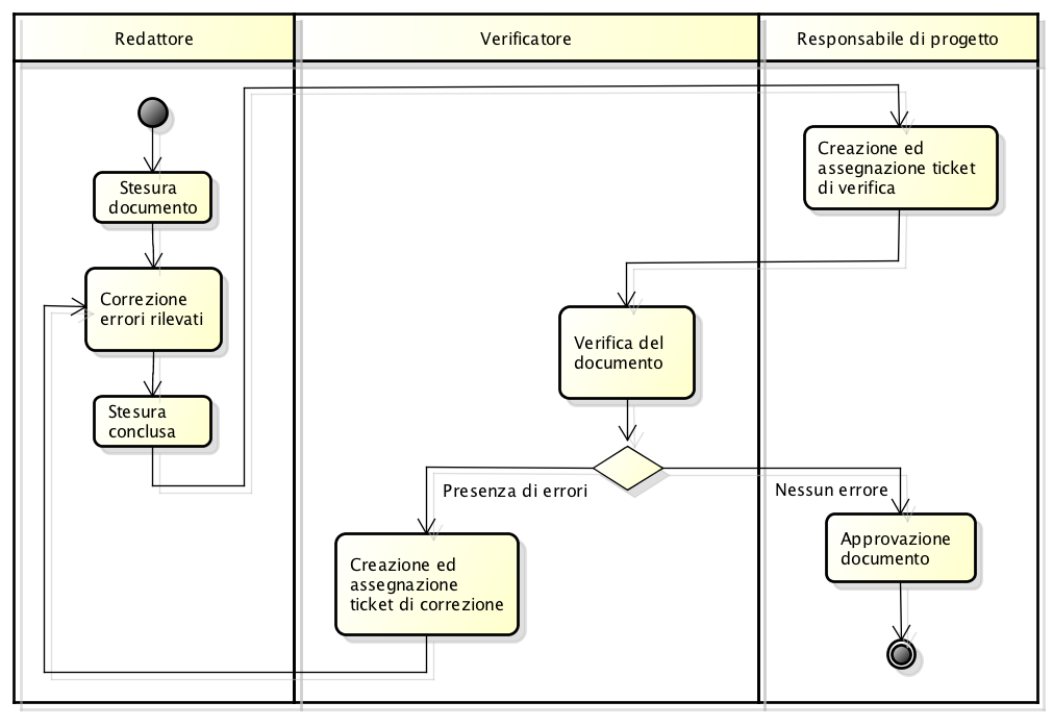
\includegraphics[width=0.9\linewidth]{img/proceduraDocumenti}
\caption[Procedura avanzamento documento]{Procedura avanzamento documento}
\label{fig:proceduraDocumenti}
\end{figure}





